%! Author = gramic
%! Date = 15.03.24

% Preamble
\begin{flushleft}
    \subsubsection{StackGres - Citus}
    \paragraph{Architektur}
    Für das Benchmarking wurde ein minimales setting ausgewählt.\\
    Ein Coordinator und einen Shard-Node mit einem Leader- und Replica-Pod.\\
    \begin{figure}[H]
        \centering
        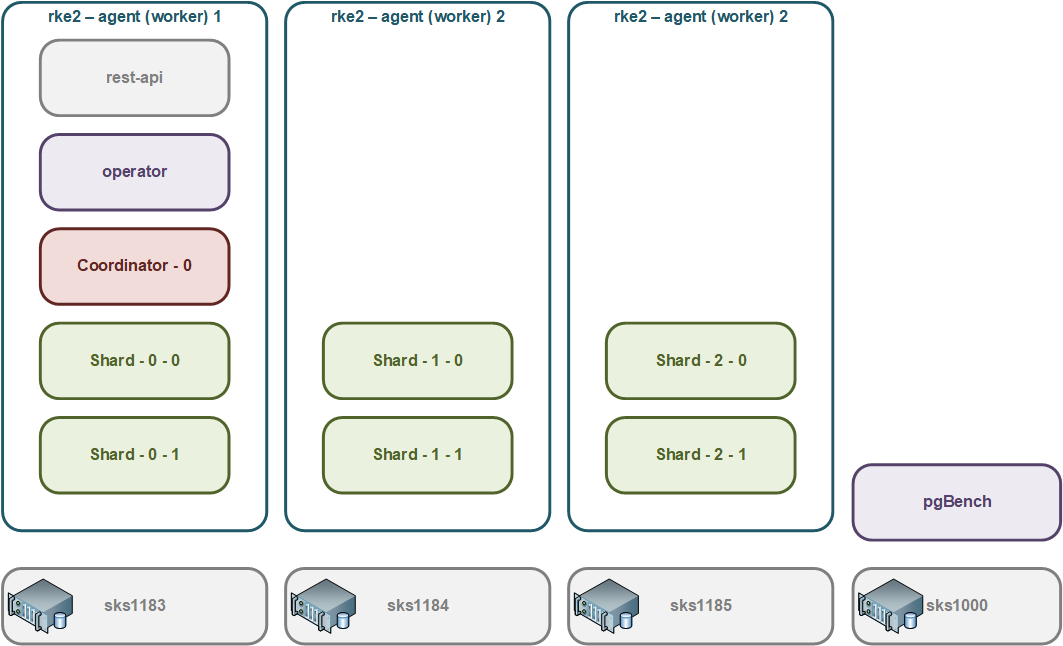
\includegraphics[width=0.8\linewidth]{source/implementation/evaluation/postgresql_ha_solutions/stackgres/stackgres-citus-evaluation-architecture}
        \caption{Stackgres - Citus - Evaluationsarchitektur Benchmarking}
        \label{fig:stackgres-citus-evaluation-architecture}
    \end{figure}
    Für die Self Healing Tests wurde eine umfangreichere Architektur vorgenommen.\\
    Es stellte sich heraus, dass man relativ leicht die beim \hyperref[subpar:citus_sharding]{Citus Sharding} beschriebene Lösung zum Replizieren leicht umzusetzen ist:
    \begin{figure}[H]
        \centering
        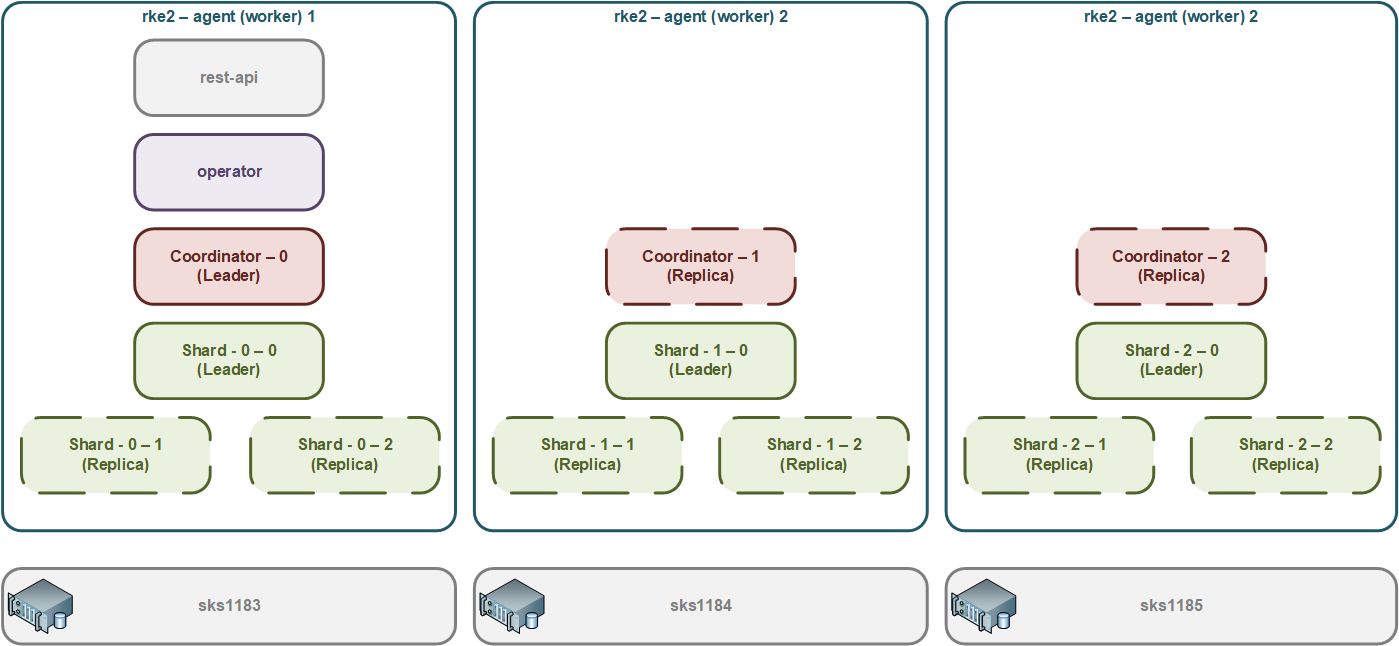
\includegraphics[width=0.8\linewidth]{source/implementation/evaluation/postgresql_ha_solutions/stackgres/stackgres_citus_architecture_self_healing_test}
        \caption{Stackgres - Citus - Evaluationsarchitektur Self Healing Tests}
        \label{fig:stackgres_citus_architecture_self_healing_test}
    \end{figure}
\end{flushleft}
\begin{flushleft}
    \paragraph{Ressourcenhunger}
    Aus den Architekturschemen ist bereits ersichtlich, dass StackGres sehr viele Pods erstellt.\\
    StackGres erzeugt mindestens einen Operator- und einen REST-API-Pod, der aber auch für das GUI verwendet wird.\\
    Nun kommt der Coordinator-Pod hinzu und je nach Auswahl pro Node ein Shard-Pod wobei es mindestens eine Instanz braucht.\\
    Will heissen, im Worst-Case sind auf einem Node mindestens 4 Pods, auf dem Server kann aber auch noch der k8s-server (control-plane) stehen.\\
    Pro Pod muss mindestens eine CPU gesetzt werden, auch der k8s-Server benötigt mindestens eine CPU, heisst das pro Server mit Minimal setting 5 CPUs benötigt werden:
    \begin{figure}[H]
        \centering
        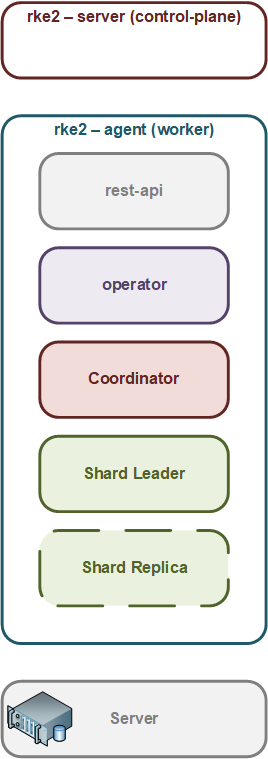
\includegraphics[width=0.1\linewidth]{source/implementation/evaluation/postgresql_ha_solutions/stackgres/stackgres_citus_architecture_resource_stack}
        \caption{Stackgres - Citus - Resourcen - Stack}
        \label{fig:stackgres_citus_architecture_resource_stack}
    \end{figure}
    Auch Memory und Storage muss eingerechnet werden, besonders wenn pro Shard noch mehrere Instanzen deployt werden sollen.
    Dazu kommt noch eine weitere eigenheit von StackGres.
\end{flushleft}
\begin{flushleft}
    Dazu kommt noch eine weitere eigenheit von StackGres.\\
    Pro Datenbank wird Standardmässig ein Cluster erstellt mit jeweils mindestens einem Coordinator und dem ganzen Stack der daran hängt:
    \begin{figure}[H]
        \centering
        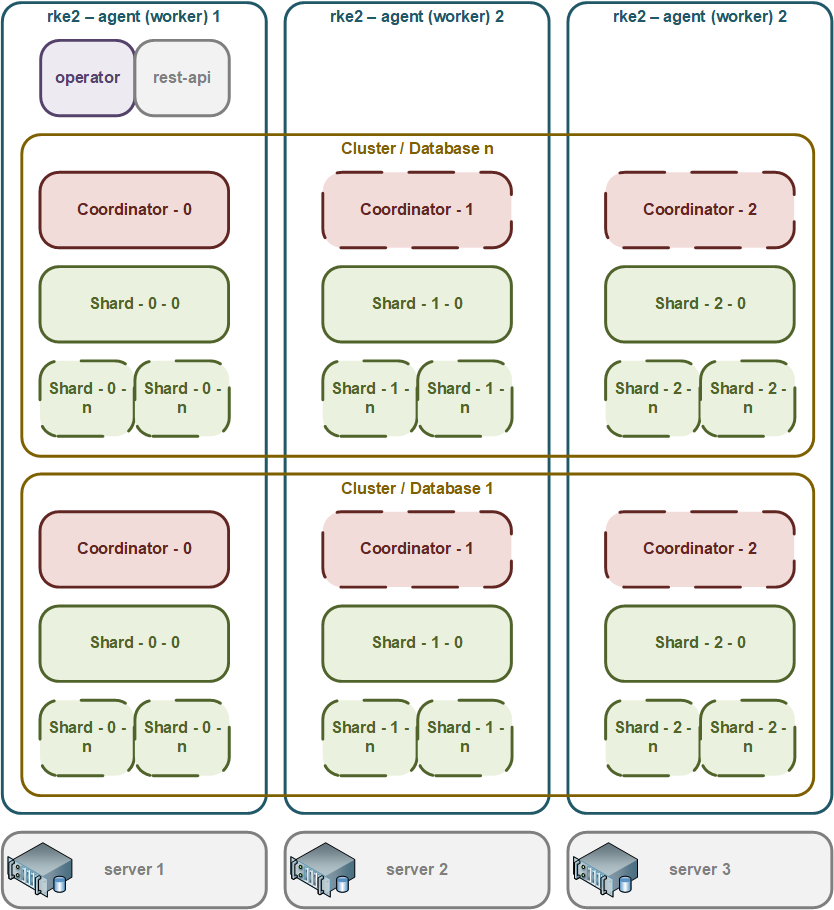
\includegraphics[width=0.1\linewidth]{source/implementation/evaluation/postgresql_ha_solutions/stackgres/stackgres_citus_architecture_clustering}
        \caption{Stackgres - Citus - Datenbank - Cluster}
        \label{fig:stackgres_citus_architecture_clustering}
    \end{figure}
    Entsprechend steigt der Ressourcenbedarf zusätzlich.
\end{flushleft}
\begin{flushleft}
    \paragraph{Installation}
    StackGres bietet von Haus aus an, einen Sharded Cluster mit Citus zu installieren.\\
    Dabei muss allerdings das StackGres Extension Repository erreichbar sein, welches mit \texttt{https} erreichbar sein muss.
\end{flushleft}
\begin{flushleft}
    Hier wird es nun knifflig sobald Proxys im Spiel sind.\\
    Selbst wenn die Proxy-Settings auf dem Host und im \gls{rke2} (\texttt{CONTAINERD\_HTTPS\_PROXY} / \texttt{CONTAINERD\_HTTP\_PROXY} / \texttt{CONTAINERD\_NO\_PROXY}) gesetzt sind,\\
    ist dies keine Garantie das mittels \texttt{https} aus dem Pod heraus kommuniziert werden kann, selbst wenn es mit \texttt{curl} möglich ist.\\
    Damit dies möglich ist, müssen die Proxy-Zertifikate auf den Host installiert werden.\\
    Alternativ kann die Kommunikation über \texttt{http} erzwungen werden.\\
    StackGres bietet diese möglichkeit und da es sich um eine Evaluationsumgebung handelt, wurde dieser Weg gewählt.\\
    Zum einen muss der Proxy nach der \texttt{proxyUrl} eingegeben werden, danach müssen die Parameter \texttt{skipHostnameVerification:true} und \texttt{setHttpScheme:true} gesetzt werden.\\
    Die Proxy-URL muss dabei wie folgt aufgebaut werden:
\lstset{style=gra_codestyle}
\begin{lstlisting}[language=yaml, caption=StackGres - values.yaml - Extension proxyUrl,captionpos=b,label={lst:stackgres_extension_proxyurl},breaklines=true]
<proxy scheme>%3A%2F%2F<proxy host>%3A<proxy port>
\end{lstlisting}
    Proxy Schema meint dabei \texttt{http} oder \texttt{https}
    Für den KSGR-Proxy sieht der gesamte String entsprechend so aus:
\lstset{style=gra_codestyle}
\begin{lstlisting}[language=yaml, caption=StackGres - values.yaml - Extension Proxy,captionpos=b,label={lst:stackgres_extension_proxy},breaklines=true]
extensions:
  repositoryUrls:
  - https://extensions.stackgres.io/postgres/repository?proxyUrl=http%3A%2F%2Fsproxy.sivc.first-it.ch%3A8080?skipHostnameVerification:true&setHttpScheme:true
\end{lstlisting}
\end{flushleft}
\begin{flushleft}
    Die Ursachenforschung hat viel Zeit in Anspruch genommen.\\
    Es sind nebst dem Versuch, eine Freigabe via Pod-Affinität zu lösen, drei Tage verstrichen bis StackGres die Extensions ausführen konnte.
\end{flushleft}
\begin{flushleft}
    Die Installation von StackGres und das anschliessende deployment von Clustern benötigt etwas mehr Schritte als bei YugabyteDB.
\end{flushleft}